\chapter{Introduction}
\label{ch:intro}

First known to be described in 3000~BC by the ancient Egyptian Edwin Smith Papyrus \cite{hajdu2011}, cancer has remained an unparalleled burden on humanity, currently accounting for the second-leading cause of death in the United States \cite{xu2020} and worldwide \cite{who_cancer_epi2018}. This remains despite centuries of medical progress and cancer research. Modern medical understanding of cancer began in the 19\textsuperscript{th} century with Dr.\ Robert Virchow's description of cancer as a malignant transformation of normal cells \cite{walter2017}. Since then, oncology (the study of cancer and practice of cancer-related medicine) has continued to accelerate, such that in 2019 the United States National Cancer Institute received \$6.1~billion in federal funds, by far the largest beneficiary of the National Institutes of Health at 15\% of all NIH funding \cite{nihbudget2000-2020}.

%second-to-last sentence: add stat about % of people dx with cancer some time in their life
Corresponding with increased interest and funding of cancer research, along with the steady march of biomedical and other fields of science, cancer survival rates have incrementally improved, most dramatically in the later 20\textsuperscript{th}~century. From 1990 to 2017, the combination of improved cancer care and reduced tobacco smoking has led to a 15\% reduction in the worldwide age-standardized cancer death rate \cite{owidcancer}, a trend particularly pronounced in lung cancer. However, as mortality from many other causes has also declined substantially during the previous century and lifespan has correspondingly increased, cancer deaths remain high, in fact increasing from 5.7~million to 8.8~million worldwide from 1990--2017 \cite{owidcancer}. Therefore, it is clear that there remains an urgent need for improved understanding, prevention, diagnosis, and treatment of this devastating and often deadly disease.

In this work, we will propose a view of cancer as a dynamic process of pathology in the human body. The infrastructure of modern medical practice divides a patient into discrete time points; for instance the timing of patient appointments, inpatient rounds, notes in a medical record, or cycles of chemotherapy or radiation therapy. Yet for the patient, cancer often constitutes a daily, moment-to-moment awareness, both a physical and mental burden of such severity that on average 13\% (and perhaps more) of cancer patients exhibit symptoms of clinical depression \cite{niedzwiedz2019}. Moreover, cancer is fundamentally moment-to-moment on the biological level, with each division of a cancer cell another opportunity for change. Therefore, we believe that a mental and scientific model of cancer as a process has potential to suggest new avenues of investigation and treatment paradigms.

In light of this model, we present studies of microsatellite instability (MSI), a phenomenon in which cancer cells mutate (acquire changes in DNA) exceptionally quickly and in highly random ways. We next provide studies of cholangiocarcinoma, interdigitating dendritic cell sarcoma, and small cell lung cancer, in which we utilize computational analysis to construct models of cancer cell evolution in time and space (from metastasis). Finally, we introduce a new mathematical approach relating MSI with models of clonal evolution, and apply this to a mixed cohort of cancers with MSI\@. All of these studies have been accepted in peer-reviewed research journals.

%paragraph introducing sections
%first, abbreviated review of DNA biology and mutations
%as genomics central to all studies here, survey of genomics
%description of tumor heterogeneity
In this introduction, we will first provide an abbreviated review of DNA biology relevant to cancer mutation. As genomic analysis is central to all of the studies we present, we will briefly survey concepts and methods essential to modern genomics. We will interrogate tumor heterogeneity in later chapters, therefore we describe the concepts of tumor heterogeneity and tumor subclones.

\section{DNA}
At the root of cellular life, including cancer, is \textbf{DNA} (deoxyribonucleic acid), therefore an understanding of its structure, functions, and potential change is essential to an understanding of cancer biology. DNA was first discovered in 1869 by Dr.\ Friedrich Miescher, and its chemical structure was elucidated in 1953 by Drs.\ James Watson and Francis Crick \cite{pray2008}. In essence, DNA contains a ``blueprint'' for a cell. As stated by Crick and termed the Central Dogma of Molecular Biology \cite{crick1970}, DNA contains chemical instructions followed by a cell for production of proteins. Proteins in turn accomplish various cellular functions. Cancer is characterized by changes in DNA, termed genetic alterations \cite{tabin1982,reddy1982}. Typically, cancers possess alterations which lead to changes in proteins themselves and/or the amounts of each protein produced such that cells divide without limit.

\subsection{Function}
\label{ssec:intro:dna_function}
DNA is an incredibly dense medium of information storage, with a peak theoretical information density of 460 exabytes per gram \cite{dong2020}. The four DNA bases can be represented with 2 bits of information apiece, therefore the 3,110,748,599 bases in the current human reference genome\footnote{Non-N bases included in genome assembly GRCh38.p13 regardless of chromosome or scaffold.} \cite{lander2001} whose sequence is known constitute \textapprox{}741.7 megabytes of information. This complex genomic information is organized at many levels. Perhaps the most useful level of organization is the \textbf{gene}, commonly defined as the instructions to build one or more related peptides, however perhaps better defined as a template for one or more \textbf{transcripts} of RNA (ribonucleic acid) \cite{pearson2006}. Genes can be divided into coding and noncoding genes. Coding genes produce transcripts termed \textbf{messenger RNAs} (mRNA) that specify a peptide sequence for protein construction. Noncoding genes produce transcripts termed \textbf{non-coding RNAs} (ncRNA) that themselves serve a biological function \cite{esteller2011}, and these in fact account for \textgreater{}~90\% of the RNA sequences transcribed from the human genome \cite{slack2019}. However, this distinction is becoming blurred by recent findings that some non-coding RNAs encode peptides and some mRNAs perform regulatory functions \cite{li2019}, and RNA biology remains a highly active field of research.

\begin{figure}[htb]
    \centering
    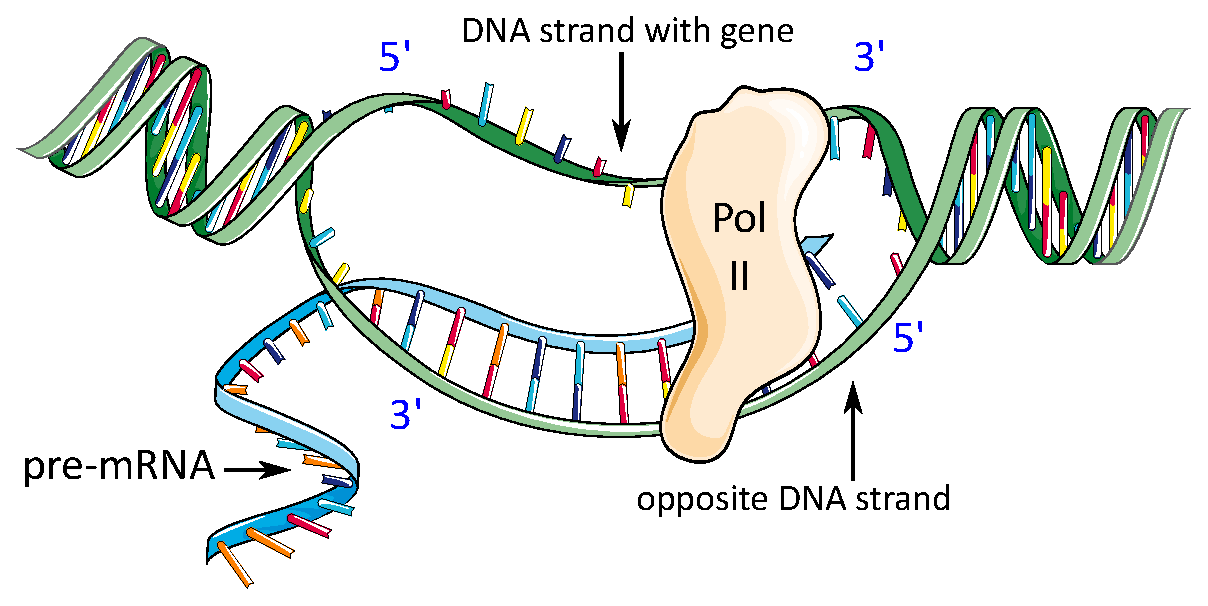
\includegraphics[width=0.75\textwidth,keepaspectratio]{images/intro/transcription}
    \caption[Illustration of DNA transcription.]{Illustration of DNA transcription by RNA Pol II to produce pre-mRNA\@. Image is adapted and altered from ``Transcription'' and ``Protein'' by Les Laboratoires Servier, licensed under CC BY 3.0 (\url{https://creativecommons.org/licenses/by/3.0/}).}
    \label{fig:intro:transcription}
\end{figure}
For coding genes, the first step in production of a peptide from a given gene is \textbf{transcription}, the production of RNA from a DNA sequence \cite{sainsbury2015}. RNA is a highly similar molecule to DNA, with the addition of a hydroxyl group to the 2' position of the pentose ring, and substitution of uracil (U) for thymine \cite{horton19_2006}. Transcription begins with recruitment of the RNA polymerase II (Pol II) enzyme by transcription factor proteins to a Transcription Start Site (TSS) region of a gene \cite{kapranov2009}. Pol II then reads a gene in the 5' to 3' direction (gene can be on either positive or negative strand), and synthesizes a fragment of RNA that is complementary to the opposite DNA strand (Figure~\ref{fig:intro:transcription}). This fragment is termed \textbf{pre-messenger RNA}, or pre-mRNA.

\begin{figure}[htb]
    \centering
    \includegraphics[width=0.6\textwidth,keepaspectratio]{images/intro/Chromosome-DNA-gene}
    \caption[High-level organization of DNA.]{High-level organization of DNA\@. DNA strands are wrapped around histone protein complexes to form nucleosomes, and entire DNA strands are termed chromosomes. DNA sequence contains genes (a feature of sequence information rather than a biochemical difference from intragenic DNA), which in turn contain introns, exons and various regulatory regions. ``Chromosome-DNA-gene'' by Thomas Splettstoesser is licensed under CC BY-SA 4.0 (\url{https://creativecommons.org/licenses/by-sa/4.0/}).}
    \label{fig:intro:dna_hierarchy}
\end{figure}
Genes contain functional regions termed \textbf{exons} and \textbf{introns} (Figure~\ref{fig:intro:dna_hierarchy}), demarcated by splice site sequences \cite{jo2015}. Exons contain instructions for sequences of amino acids to build peptides. Introns do not, but may serve regulatory and other functions. The next step in peptide production is splicing, in which a collection of proteins and functional RNA molecules termed the spliceosome excises introns from the pre-mRNA fragment \cite{will2011}. After addition of a 5' altered guanine cap \cite{shatkin1976} and a 3' poly-adenine tail \cite{guhaniyogi2001}, the new messenger RNA molecule is exported from the nucleus to the cytoplasm. By varying the exons that are included, one gene is able to produce multiple different mRNA molecules termed transcripts, each of which codes for a different peptide.

The mRNA is then processed by the ribosome, which assembles a peptide sequence based on the mRNA sequence \cite{horton19_2006}. This is termed \textbf{translation}. Three-letter sequences, termed \textbf{codons}, specify particular amino acids to be included in the peptide \cite{nirenberg2004}. Three of the 64 codons (UAA, UAG, UGA), termed stop codons, signal the ribosome to cease addition of amino acids and release the produced peptide. Ribosomes provide a scaffold for amino acid-bearing transfer RNA (tRNA) molecules complementary to each codon, and catalyze peptide bonds between newly arriving amino acids and the growing polypeptide chain \cite{steitz2008}. Peptides may undergo an enormous variety of additional post-translational modifications and other processing to produce mature and properly folded proteins \cite{conibear2020}.

Non-coding RNAs are also transcribed from the genome (potentially by different RNA polymerases \cite{turowski2016}) and may undergo splicing \cite{krchnakova2018} along with various other mechanisms of post-transcriptional modification \cite{leighton2018}. However these RNA molecules are not translated into peptides, rather they perform biological functions of their own. Also unlike mRNA, ncRNA is not always exported into the cytoplasm as some ncRNAs fulfill functions in the nucleus. Several classes of ncRNAs exist, such as micro RNAs (miRNA) which typically target complementary mRNA sequences for degradation to reduce expression of these genes, the aforementioned tRNAs essential to mRNA translation, ribosomal RNA (rRNA) which contributes to the ribosome structure, and long non-coding RNAs (lncRNA) which serve a variety of functions \cite{slack2019}.

Many DNA regions have regulatory functions instead of or in addition to serving as a template for RNA production. Critical to cell function, growth, and differentiation is \textbf{gene regulation}, or the ability of the cell to control the quantity of each protein it is capable of producing \cite{guo2014}. The relative amount of a gene or transcript's transcription is known as its expression. Cells of different types must express different genes to perform their various functions, and cells must alter expression in response to environmental or other stimuli. This is facilitated by the instability of mRNA in the cytoplasm (half-life highly variable but median \textapprox{}10~hours) \cite{yang2003}, therefore cells must continuously produce mRNA to maintain high expression, which grants them the ability to quickly reduce gene expression on demand. Increased expression is termed upregulation, and decreased expression downregulation.

A variety of mechanisms to regulate transcription are known, with three of the most important being DNA methylation, histone modification, and transcription factors. Methylation of the 5' position of cytosine to form 5-methylcytosine, particularly at cytosines followed by guanine (CpG), is known to repress transcription \cite{jin2011}. Histone proteins electrostatically adhere to DNA due to their positive charge. This interaction can be altered by modifying exposed histone residues along with substitution of variant histone proteins \cite{greer2012,ernst2010,bonneville2012}. For instance, histone acetylation (adding a negatively-charged functional group) tends to increase gene expression by decreasing the histone positive charge \cite{eberharter2002}, facilitating access to DNA by RNA Pol II and other enzymes involved in transcription. \textbf{Transcription factors} constitute a large family of proteins which bind to DNA regions called enhancers and recruit other DNA-binding proteins and transcriptional enzymes \cite{spitz2012}. These various mechanisms of DNA regulation constitute an essential component of the fantastically complex system that is the human cell.

\subsection{Replication}
\label{ssec:intro:dna_replication}
It is insufficient for cells to merely use DNA as a blueprint; in order to divide and produce new cells, the cell must copy its entire genome with high fidelity. This occurs during the S (synthesis) phase of the cell cycle, and requires a complicated assortment of proteins known as the \textbf{replisome} \cite{bellelli2020}. Given this complexity, we will only briefly outline the major events of DNA replication.

\begin{figure}[htb]
    \centering
    \includegraphics[width=0.9\textwidth,keepaspectratio]{images/intro/0323_DNA_Replication_altered}
    \caption[High-level illustration of DNA replication.]{High-level illustration of DNA replication. ``DNA Replication'' \cite{betts2013} by OpenStax is licensed under CC BY 4.0 (\url{https://creativecommons.org/licenses/by/4.0/}), and has been modified to highlight the DNA region being replicated and alter labels.}
    \label{fig:intro:replication_schematic}
\end{figure}
A single replisome is able to assemble 50 nucleotides per second \cite{chali1_2014}, which by itself would take over two years to replicate the entire human genome. To facilitate replication in a reasonable time frame, multiple replisomes assemble at sites termed replication origins (ori)\footnote{Though DNA synthesis occurs during the S phase, oris were `licensed' during G\textsubscript{1}.} and replicate the genome in parallel \cite{bellelli2020}. At the beginning of the S phase, the CMG helicase complex ``unzips'' the DNA double helix beginning at an ori to create a replication fork, and replication protein A (RPA) binds to the exposed DNA single strands (Figure~\ref{fig:intro:replication_schematic}). RPA recruits a replisome on each strand, and both replisomes traverse the strand in the 3'\textrightarrow{}5' direction, \textit{i.e.}\ away from the ori in opposite directions. In the replisome, DNA polymerase $\alpha$ (POL$\alpha$) lays down a short primer sequence, which is extended by POL$\varepsilon$ to create a new DNA strand termed the leading strand (extending in the 5'\textrightarrow{}3' direction), complementary to the original DNA single strand being traversed. Such strand extension entails adding nucleotides one at a time through phosphate linkages from the 3' hydroxyl group of the preceding nucleotide to the 5' hydroxyl of the new nucleotide. Meanwhile, POL$\delta$ synthesizes short DNA fragments (called Okazaki fragments) in the other direction (towards the ori) \cite{langston2006}, 3'\textrightarrow{}5' traversing the opposite source strand. Okazaki fragments are ligated to create a continuous DNA strand, called the lagging strand. Replication continues until the replisome encounters another replisome (from another ori), and CMG is disassembled to permit new double helices to form. Each new double-stranded DNA molecule contains one original strand and one newly synthesized, complementary strand. The end result of this process is two identical copies of the original genome, which will be equally divided among daughter cells during the M phase of the cell cycle.

Of interest, the machinery of DNA replication can be exploited \textit{in vitro} to ``amplify'' (extensively copy) a DNA sequence in a process termed polymerase chain reaction, or PCR \cite{bartlett2003}. This process utilizes RNA primers complementary to sequences flanking the sequence of interest, along with a thermostable DNA polymerase (typically isolated from extremophile bacteria) and deoxynucleotide triphosphate molecules (dNTPs, which have a chain of 3 phosphate groups linked to the deoxyribose 5' hydroxyl group) \cite{green2018}. In each PCR cycle, the solution is heated to separate double-strand DNA fragments into single strands, and cooled to permit new primer binding and for DNA polymerase to synthesize new complementary strands. Through repeated cycles, this reaction can geometrically increase the number of identical (except for polymerase errors) DNA fragments. PCR is used extensively throughout molecular biology, including detection of DNA sequences through quantification of DNA yields at each cycle (termed quantitative PCR or qPCR), and generation of the relatively large quantities of DNA typically necessary for sequencing.

\subsection{Mutation}
\label{ssec:intro:mutation}
A variety of events and mechanisms can lead to changes in a DNA sequence, which are termed \textbf{mutations} \cite{lodish2000}. In healthy human cells, mutations have been estimated to occur at a rate of $6 \times 10^{-11}$ per base per cell division \cite{lynch2010}, or roughly an average of one mutation per every five cell divisions. Depending on a mutation's position and the bases affected, mutations can give rise to phenotypes (effects of a gene) ranging from nonexistent to catastrophic, or even in rare cases beneficial. The possibility of mutations is therefore a double-edged sword; necessary for evolution, yet creating the possibility of deleterious mutations that lead to genetic disorders including cancer \cite{loewe2010}.

The most common forms of mutation affect one or a few bases. A change of a single base is termed a \textbf{single nucleotide variant} (SNV) \cite{katsonis2014}. A change of a purine to another purine, or a pyrimidine to another pyrimidine, is termed a \textbf{transition}. A change of a purine to a pyrimidine, or vice versa, is a \textbf{transversion}. If in a coding region of the genome, it may be \textbf{synonymous} or \textbf{nonsynonymous}. As there are 64 possible three-letter codons for 20 amino acids, the genetic code contains redundancy. Therefore, some SNVs do not change the protein product and are termed synonymous or silent, however in rare cases even synonymous SNVs may have phenotypic effects \cite{zheng2014}. Nonsynonymous SNVs do change the protein product, and can be further subdivided into \textbf{missense} or \textbf{nonsense}. Missense mutations change one amino acid codon or stop codon into another amino acid. Nonsense mutations change an amino acid codon into a premature stop codon, typically leading to a truncated and nonfunctional protein product \cite{jopling2014}. Insertions and deletions of bases can also happen, collectively termed \textbf{indels} for changes \textless{}~1000~bp \cite{sehn2015}. In coding regions, these can be classified as \textbf{frameshift} or \textbf{non-frameshift} indels. As translation occurs three letters of DNA at a time (the choice of first, second, and third bases termed the frame), addition or removal of a non-multiple of 3 bases disrupts translation of all downstream amino acids, usually with severe consequences for the protein. Non-frameshift indels affect multiples of 3 bases, therefore preserving the frame and downstream amino acids (unless a stop codon is inserted).

Cancers can possess a variable quantity of SNVs and indels, termed the \textbf{tumor mutation burden} (TMB) \cite{merino2020}. TMB is typically quantified as the number of detected mutations divided by the panel size in megabases. Though there is currently not a universal standard for TMB classification, tumors with TMB $\ge 10$ are often considered ``hypermutated'' or TMB-high (TMB-H) \cite{shao2020,keytrudafda2017}, with other tumors classified as TMB-low. Hypermutation is known to occur through a variety of mechanisms \cite{campbell2017}.

\begin{figure}[htb]
    \centering
    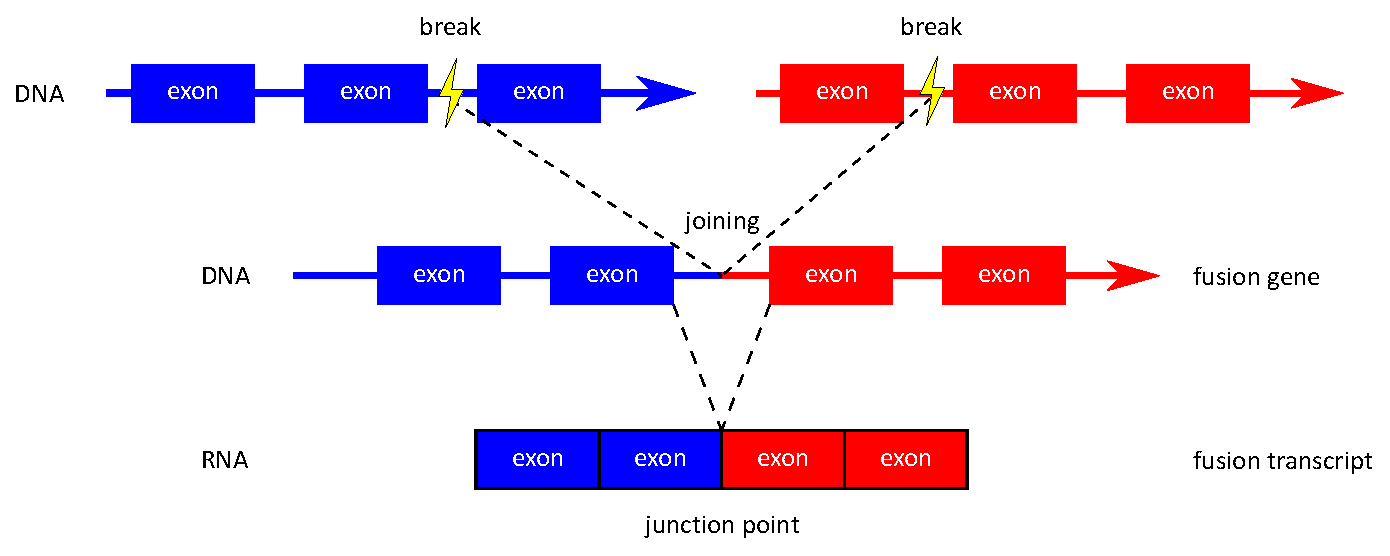
\includegraphics[width=0.9\textwidth,keepaspectratio]{images/intro/fusion_example}
    \caption[Illustration of a gene fusion.]{Illustration of a gene fusion. Double-strand breakage of at least one site creates free-floating fragments of DNA, which may rejoin new locations of chromosomes (either another breakage site as depicted here, or a chromosome end). If this occurs between coding genes, a new fusion gene is produced containing sequence from both partner genes. This may include exons and introns, giving rise to new fusion transcripts.}
    \label{fig:intro:fusion_schematic}
\end{figure}
Mutations can also affect larger DNA regions, up to and including entire chromosomes \cite{hastings2009}. Large DNA regions ($\ge 1000$~bp) can be gained or lost, a phenomenon termed \textbf{copy number variation} (CNV)\@. Copy number gains increase the number of copies of affected genes, which in term increases their expression as more mRNA can be synthesized in parallel. Loss of one copy of a gene can reduce its expression, and losing both copies (or a singular copy on a sex chromosome in a male) deletes the gene entirely from the cell. Another type of large DNA alteration is \textbf{rearrangement}, in which DNA strands are broken and recombine in new ways to form altered chromosomes \cite{hasty2014}. When breakpoints occur within or near genes, rearrangements can give rise to \textbf{gene fusions} \cite{rabbitts1994,osborne2007}, or new genes containing components of what were originally two (or rarely more) separate genes (Figure~\ref{fig:intro:fusion_schematic}). Such fusion genes may exert different effects than either of the original partner genes.

A wide variety of mechanisms for DNA mutation are known \cite{chakarov2014}. Mutational mechanisms can be divided into \textbf{exogenous mechanisms}, which originate outside the cell, and \textbf{endogenous mechanisms}, originating within the cell. Exogenous mechanisms include chemical agents termed \textbf{mutagens} \cite{benigni2011}, as well as environmental stressors such as ultraviolet light \cite{pfeifer2005} and ionizing radiation \cite{little2000}. Many endogenous mechanisms are known, therefore we will only describe some major mutational mechanisms (exogenous and endogenous) which are referenced in later chapters.

Tobacco smoke is well-known to be associated with cancer \cite{obe1984}, and contains multiple mutagens. Of particular interest are polycyclic aromatic hydrocarbons, especially benzopyrene \cite{demarini2004}. Benzopyrene is converted into an epoxide derivative by cytochrome P450 (CYP) family enzymes, and in turn binds to guanine in DNA \cite{iarc2012}. These large chemical groups disrupt the normal DNA double helix structure, producing a variety of SNVs, indels, and DNA breaks which lead to rearrangements \cite{cosmic_ms}. Many chemotherapeutic agents used to treat cancer are in fact mutagens, exploiting the increased sensitivity of dividing cells to disruption of DNA synthesis \cite{ferguson1996}. For instance, molecules of platinum-based agents (\textit{e.g.}\ cisplatin, carboplatin, oxaliplatin) can bind to multiple DNA bases, cross-linking DNA strands and interfering with DNA function and replication \cite{chen2013}, which introduces characteristic patterns of mutations \cite{pich2019}. Other agents such as gemcitabine and 5\nobreakdash-fluorouracil mimic building blocks of DNA\@. Gemcitabine masquerades as cytosine and is inserted into DNA, causing DNA polymerase to stall and truncating DNA strands. 5\nobreakdash-fluorouracil mimics uracil and blocks thymine synthesis, both preventing new DNA production during cell division and inducing T\textgreater{}G transversions \cite{christensen2019}.

Ultraviolet radiation (UV) is able to directly affect nucleotides. UVA (320--400~nm) oxidizes other cellular molecules to create oxygen free radicals, which react with guanine in particular to form 8-oxoguanine \cite{kielbassa1997}. UVB (280--320~nm) and UVC (200--280~nm) attack adjacent pyrimidine bases (\textit{e.g.}\ \texttt{CC} or \texttt{CT} sequences) in a cyclization reaction (occurring at their 5-6 position double bond) which cross-links the bases. Ionizing radiation directly attacks DNA causing double-strand breaks, and also creates DNA-damaging oxygen free radicals \cite{santivasi2014}. In addition, cytosine and 5-methylcytosine are prone to spontaneously deaminate to uracil and thymine respectively (conversion of 4 position amine group to carbonyl), which causes C\textgreater{}T transitions \cite{lewis2016}. Such mutations produce a characteristic age-associated pattern termed ``clock-like'' mutation \cite{alexandrov2015}.

\begin{figure}[htb]
    \centering
    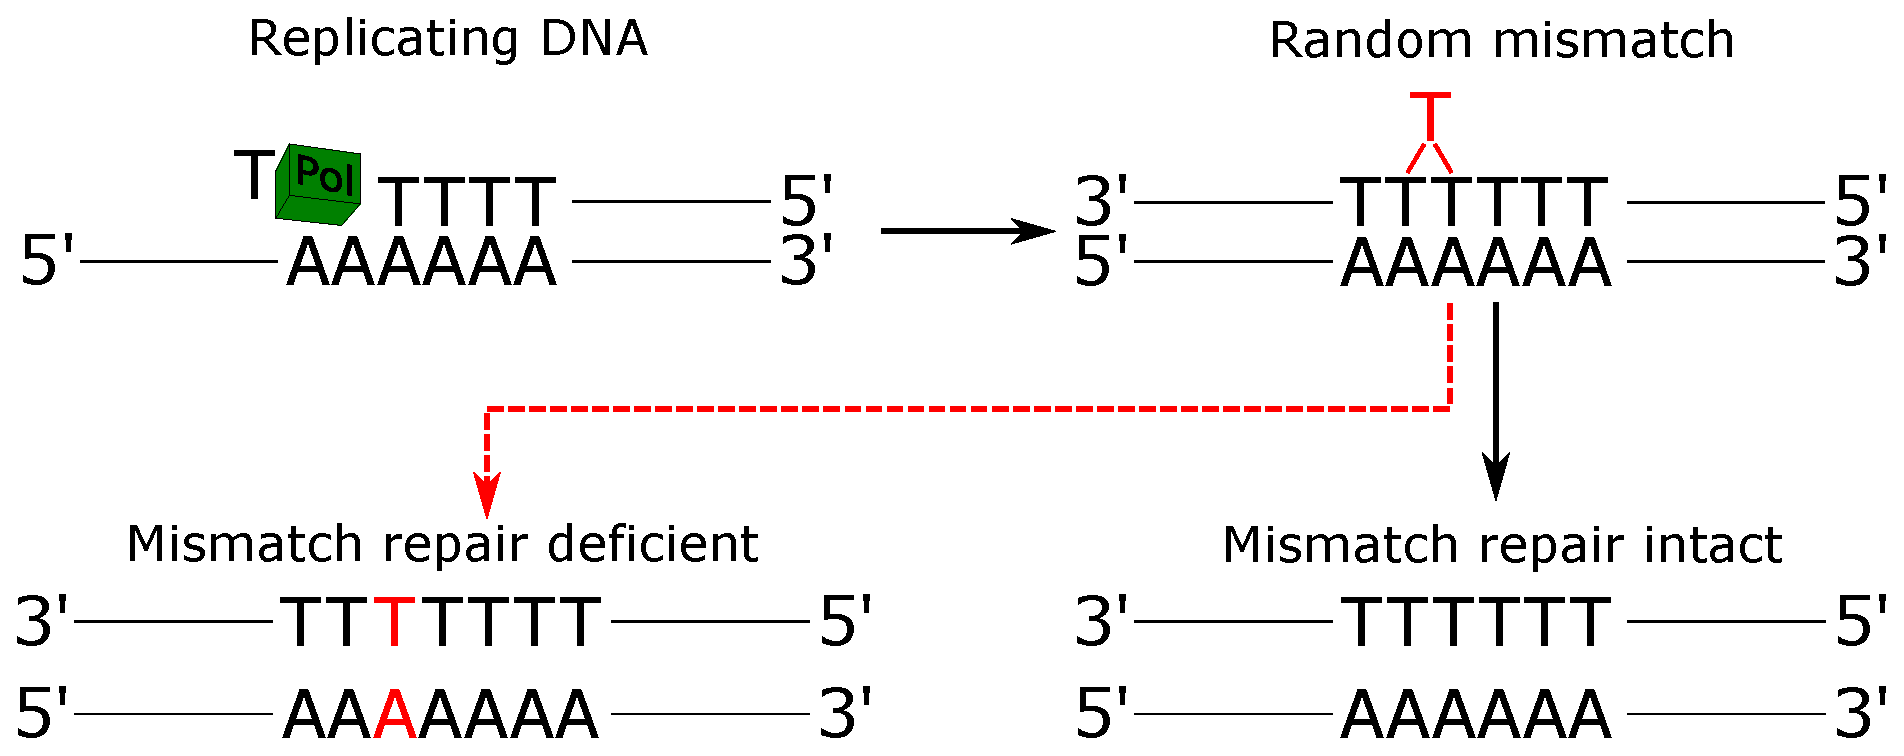
\includegraphics[width=0.9\textwidth,keepaspectratio]{images/intro/msi_schematic}
    \caption[Mechanism of microsatellite instability.]{Mechanism of microsatellite instability. Microsatellites are highly repetitive sequences which are prone to slippage during DNA replication. Failure of the mismatch repair system to repair such slippage results in random changes in the microsatellite sequence length. Reprinted by permission from Springer Nature: Springer, Detection of Microsatellite Instability Biomarkers via Next-Generation Sequencing, by Bonneville R, Krook MA, Chen HZ, Smith AM, Samorodnitsky E, Wing MR, Reeser JW, Roychowdhury S\@. \textcopyright{} 2020. \url{https://link.springer.com/protocol/10.1007\%2F978-1-4939-9773-2_5}.}
    \label{fig:intro:msi_schematic}
\end{figure}
Another mutational mechanism important in cancer is \textbf{microsatellite instability} (MSI). Microsatellites are short stretches of DNA composed of repeats of a 1--6~bp sequence (termed a motif) \cite{kelkar2010}. During DNA replication, a new strand of DNA that is slightly offset from the original sequence will still possess a high degree of complementarity, as most of the repetitive bases will still match \cite{levinson1987}. This permits DNA polymerases to ``slip'' (Figure~\ref{fig:intro:msi_schematic}), inserting or deleting copies of the motif and generating indel mutations (most microsatellites have 1~bp motifs) \cite{schloetterer1992}. MSI is one source of hypermutation, and will be discussed in further detail in Chapters \ref{ch:msilandscape} and \ref{ch:msiclones}. In addition, cells have evolved the \textbf{APOBEC} (Apolipoprotein B mRNA Editing Catalytic Polypeptide-like) family of nucleic acid editing proteins, \textit{i.e.}\ proteins with the primary (and counter-intuitive) function of \emph{inducing} mutations \cite{salter2016}. Some APOBEC members target DNA, either to facilitate somatic hypermutation in B cells\footnote{Recently, this has been disputed in favor of a reverse transcriptase-based mechanism \cite{steele2016}.} necessary to increase the variety of antibodies produced, or to scramble viral DNA.

\subsection{Repair}
%add stuff like Lynch syndrome here
With the many opportunities for mutation afforded by exogenous and endogenous mechanisms, the human cell is able to suppress mutations such that a single zygote can give rise to the \textapprox{}$3.7 \times 10^{13}$ cells in the average adult human body without incident \cite{bianconi2013}. This occurs by a variety of \textbf{repair mechanisms} \cite{chatterjee2017}, a few of which will be outlined here. Additionally, the cell has failsafe mechanisms that allow a cell to essentially self-destruct (termed \textbf{apoptosis}) if mutations are irreparable.

DNA repair begins with the polymerases during DNA replication, most of which (including POL$\varepsilon$ and POL$\delta$) have \textbf{proofreading} capabilities \cite{albertson2006}. This typically consists of a 3'\textrightarrow{}5' exonuclease domain, which removes newly added bases in response to incorrect nucleotide pairing with the original strand \cite{bebenek2018}. Other, non-polymerase exonucleases assist in proofreading \cite{mason2012}. Proofreading reduces the polymerase error rate by a hundred to a thousand-fold. Of note, some cancers acquire mutations in the proofreading domain of POL$\varepsilon$, leading to acquisition of substantial hypermutation \cite{schlesner2015}. POL$\varepsilon$-mutant cancers are often ultra-hypermutated (TMB $\ge 100$ muts/Mb) \cite{campbell2017}.

Also serving to correct replication errors is the \textbf{mismatch repair} (MMR) system, which detects and corrects DNA polymerase slippage \cite{baretti2018} (Figure~\ref{fig:intro:msi_schematic}). This system consists primarily of the MLH1/MSH2 and MSH6/PMS2 heterodimers, and also involves several additional proteins within the MSH and MLH families \cite{fishel2015}. It is believed that MSH proteins traverse newly synthesized DNA to ``scan'' it for the increased molecular flexibility which indicates a mismatch (due to its weaker affinity for the correct base's complement). Upon encountering a mismatch, more MSH protein copies are recruited to the site, followed by other proteins (including MLH family proteins) which excise a region of the new DNA strand around the mismatch. The single-strand gap is then filled in by a DNA polymerase.

Most important to repair of DNA damage is \textbf{base excision repair} (BER) \cite{zharkov2008}. Briefly, a family of 11 DNA glycosylases is responsible for patrolling DNA to identify various lesions, including but not limited to alkylated and oxidized bases \cite{krokan2013}. Although differing in details, when encountering a lesion the DNA glycosylase excises the damaged base, the deoxyribose is removed by either APE1 or POL$\beta$, and $POL\beta$ replaces the nucleotide \cite{wallace2014}. BER is also important for repair of single-strand DNA breaks. These are detected by the PARP1 and PARP2 proteins, which recruit BER enzymes including XRCC1 to trim damaged bases at the break ends and facilitate reconstitution of the strand.

BER is limited in that it can only recognize a fixed subset of DNA damage mechanisms. The \textbf{nucleotide excision repair} (NER) pathway provides a more general means of DNA sequence repair, capable of recognizing DNA lesions which distort the double helix \cite{spivak2015}. NER is also capable of detecting some forms of damage that affect multiple bases, for instance UV-induced pyrimidine dimerization. NER begins through either the transcription-coupled repair or the global genomic repair sequence. In transcription-coupled repair, DNA lesions which block RNA Pol II progression cause the polymerase to dissociate from DNA and recruit NER enzymes including TFIIH\@. In global genomic repair, double helix distortions are recognized by the XPC-hRAD23b-CETN2 complex (possibly with the help of the XPE-DDB1 complex), which recruits TFIIH\@. Other XP family proteins proceed with the repair. First, \textapprox{}30~bp around the lesion are unwound. Next, the intact DNA on the complementary strand is protected by RPA and the damaged section is excised. Finally, the gap is filled by a DNA polymerase \cite{marteijn2014}.

Cells also possess two mechanisms of double-stranded break (DSB) repair; \textbf{homologous recombination} (HR) and \textbf{non-homologous end joining} (NHEJ) \cite{mladenov2016}. HR depends on the presence of a second genome copy, therefore can only function after the S phase \cite{li2019_hr}. In this pathway, DSB are recognized by the MRN protein complex (consisting of MRE11, RAD50 and NBS1), which then trims the break ends to produce single-strand overhangs. These overhangs then invade the intact genome and DNA polymerases reconstruct the original sequence across the breakpoint using the intact genome as a reference. In contrast, NHEJ can function throughout the cell cycle, however without a second genome copy it cannot faithfully recover the sequence at the breakpoint which leads to random mutations\footnote{The relative accuracy of HR and NHEJ has been disputed, with findings of high HR error rates \cite{rodgers2015} and accurate NHEJ \cite{betermier2014}.} \cite{davis2013}. In this pathway, DSB are recognized by the Ku70/Ku80 heterodimer, which binds to both break ends to stabilize the site. Ku70/Ku80 recruits a variety of proteins, including TdT (terminal deoxynucleotidyl transferase) which adds random nucleotides to a DNA fragment \cite{boubakour2012}, and POL$\lambda$ which is capable of synthesizing short DNA fragments without a template (and hence unlikely to match the former sequence) \cite{ramadan2004}. After the break ends have been appropriately prepared, they are ligated by DNA ligase IV and Ku70/Ku80 is ubiquitinylated and degraded.

Despite these and other DNA repair mechanisms, not all mutations can be adequately repaired. Most mutations are of little to no consequence \cite{nei2010}, for instance mutations affecting intragenic regions (the stretches of DNA in between genes) or silent mutations and which do not happen to be in a region important for gene regulation. However, given the risk of mutations inducing cancer, cells have mechanisms to induce apoptosis should DNA repair fail or in the case of overwhelming DNA damage. One such mechanism involves the protein \textbf{p53} \cite{schlereth2010}, encoded by the gene \textit{TP53}. This protein is involved in multiple repair pathways including BER, NER and DSB repair \cite{offer2002}. Upon detection of DNA damage, p53 binds to p21, and p21 inhibits the cyclin~E/Cdk2 and cyclin~D/Cdk4 complexes to cause G\textsubscript{1} cell cycle arrest, along with downregulation of cdc25C expression to arrest a cell at G\textsubscript{2}/M \cite{chen2016}. If p53 remains activated for a sufficient time (because DNA repair has not concluded), it upregulates pro-apoptotic proteins such as the BH3-only protein family which attacks the mitochondrial outer membrane, leading to a cascade of events culminating in death of the cell.

\section{Overview of genomics}
\label{sec:intro:genomics}
Realization of the central role of DNA in the composition and function of an organism has led to the field of \textbf{genomics}, or study of genomes \cite{delgiacco2012}. As we have seen, genomes carry information in their sequence of nucleotides (Section~\ref{ssec:intro:dna_function}). Therefore, at the core of genomics is DNA sequencing, or the elucidation of DNA sequence \cite{weissenbach2016}. In turn, the ever-increasing quantities of data generated by sequencing methodologies has spurred developments in \textbf{bioinformatics}, the computational study of biological data. Genomics has yielded substantial insights with clinical relevance, especially in oncology \cite{shendure2019}.

\subsection{Beginnings}
\label{ssec:intro:seq_beginnings}
\begin{figure}[htb]
    \centering
    \includegraphics[width=0.9\textwidth,keepaspectratio]{images/intro/sanger_sequencing}
    \caption[High-level illustration of Sanger sequencing.]{High-level illustration of Sanger sequencing. Dideoxynucleotide triphosphate (ddNTP) molecules induce random termination of complementary strand synthesis, producing a distribution of fragments of different lengths (left). These fragments are size-sorted by gel electrophoresis (center). The particular ddNTP is determined for each fragment size, and the reverse complement of the ddNTP sequence yields the original DNA sequence. Figure by Wen and Zhong \cite{wen2019} is licensed under CC BY-NC-SA 3.0 (\url{https://creativecommons.org/licenses/by-nc-sa/3.0/}).}
    \label{fig:intro:sanger_schematic}
\end{figure}
After early experiments in sequencing of short RNA fragments \cite{minjou1972}, Sanger \textit{et al} developed the first practical method of sequencing genes and larger regions \cite{sanger1977,sanger1978}. This method, today termed Sanger sequencing, makes use of dideoxynucleotides which lack 3' hydroxyl groups. In current practice, each of the four dideoxynucleotides is typically labeled with a different fluorophore. Similarly to a PCR experiment (Section~\ref{ssec:intro:dna_replication}), primers and a DNA polymerase are added to a solution containing the DNA of interest, however dideoxynucleotide triphosphate molecules (ddNTPs) are added as well as dNTPs. DNA polymerase stops after inclusion of a dideoxynucleotide due to its inability to accept a 3' phosphate linkage. Therefore, Sanger sequencing yields a collection of fragments of different lengths, including many incomplete fragments ending in a single dideoxynucleotide (Figure~\ref{fig:intro:sanger_schematic}). These fragments are then stratified by length via gel electrophoresis, and the attached fluorophore is read to determine the identity of the base at the position given by the fragment length. Although Sanger sequencing has today largely been supplanted by newer methods, it remains in use for small-scale sequencing and as a method for validating genetic findings revealed by other sequencing methods.

Since its discovery, Sanger sequencing was applied to increasingly larger genes and genomes \cite{shendure2017}. As sequencing increased in scale, interest grew in the prospect of sequencing an entire human genome, leading to the formation of the Human Genome Project in 1990 \cite{green2015}. Its goals were to produce an entire human genome sequence by 2005 with a total budget of \$3~billion \cite{sawicki1993}. This would entail so-called ``shotgun sequencing''; creating overlapping clones of short human genome fragments which would be Sanger sequenced. The fragments would then be computationally stitched together and localized to a human genome region based on ``anchor'' regions of previously known sequence and position. During the 1990s, several improvements were made to Sanger sequencing (particularly increased automation), however a computational breakthrough by Celera, Inc.\ reduced the need for anchor regions and led to the Project's completion in 2001 \cite{venter2001}, four years ahead of schedule and \$300~million under budget \cite{kling2005,gyles2008}.

\begin{figure}[htb]
    \centering
    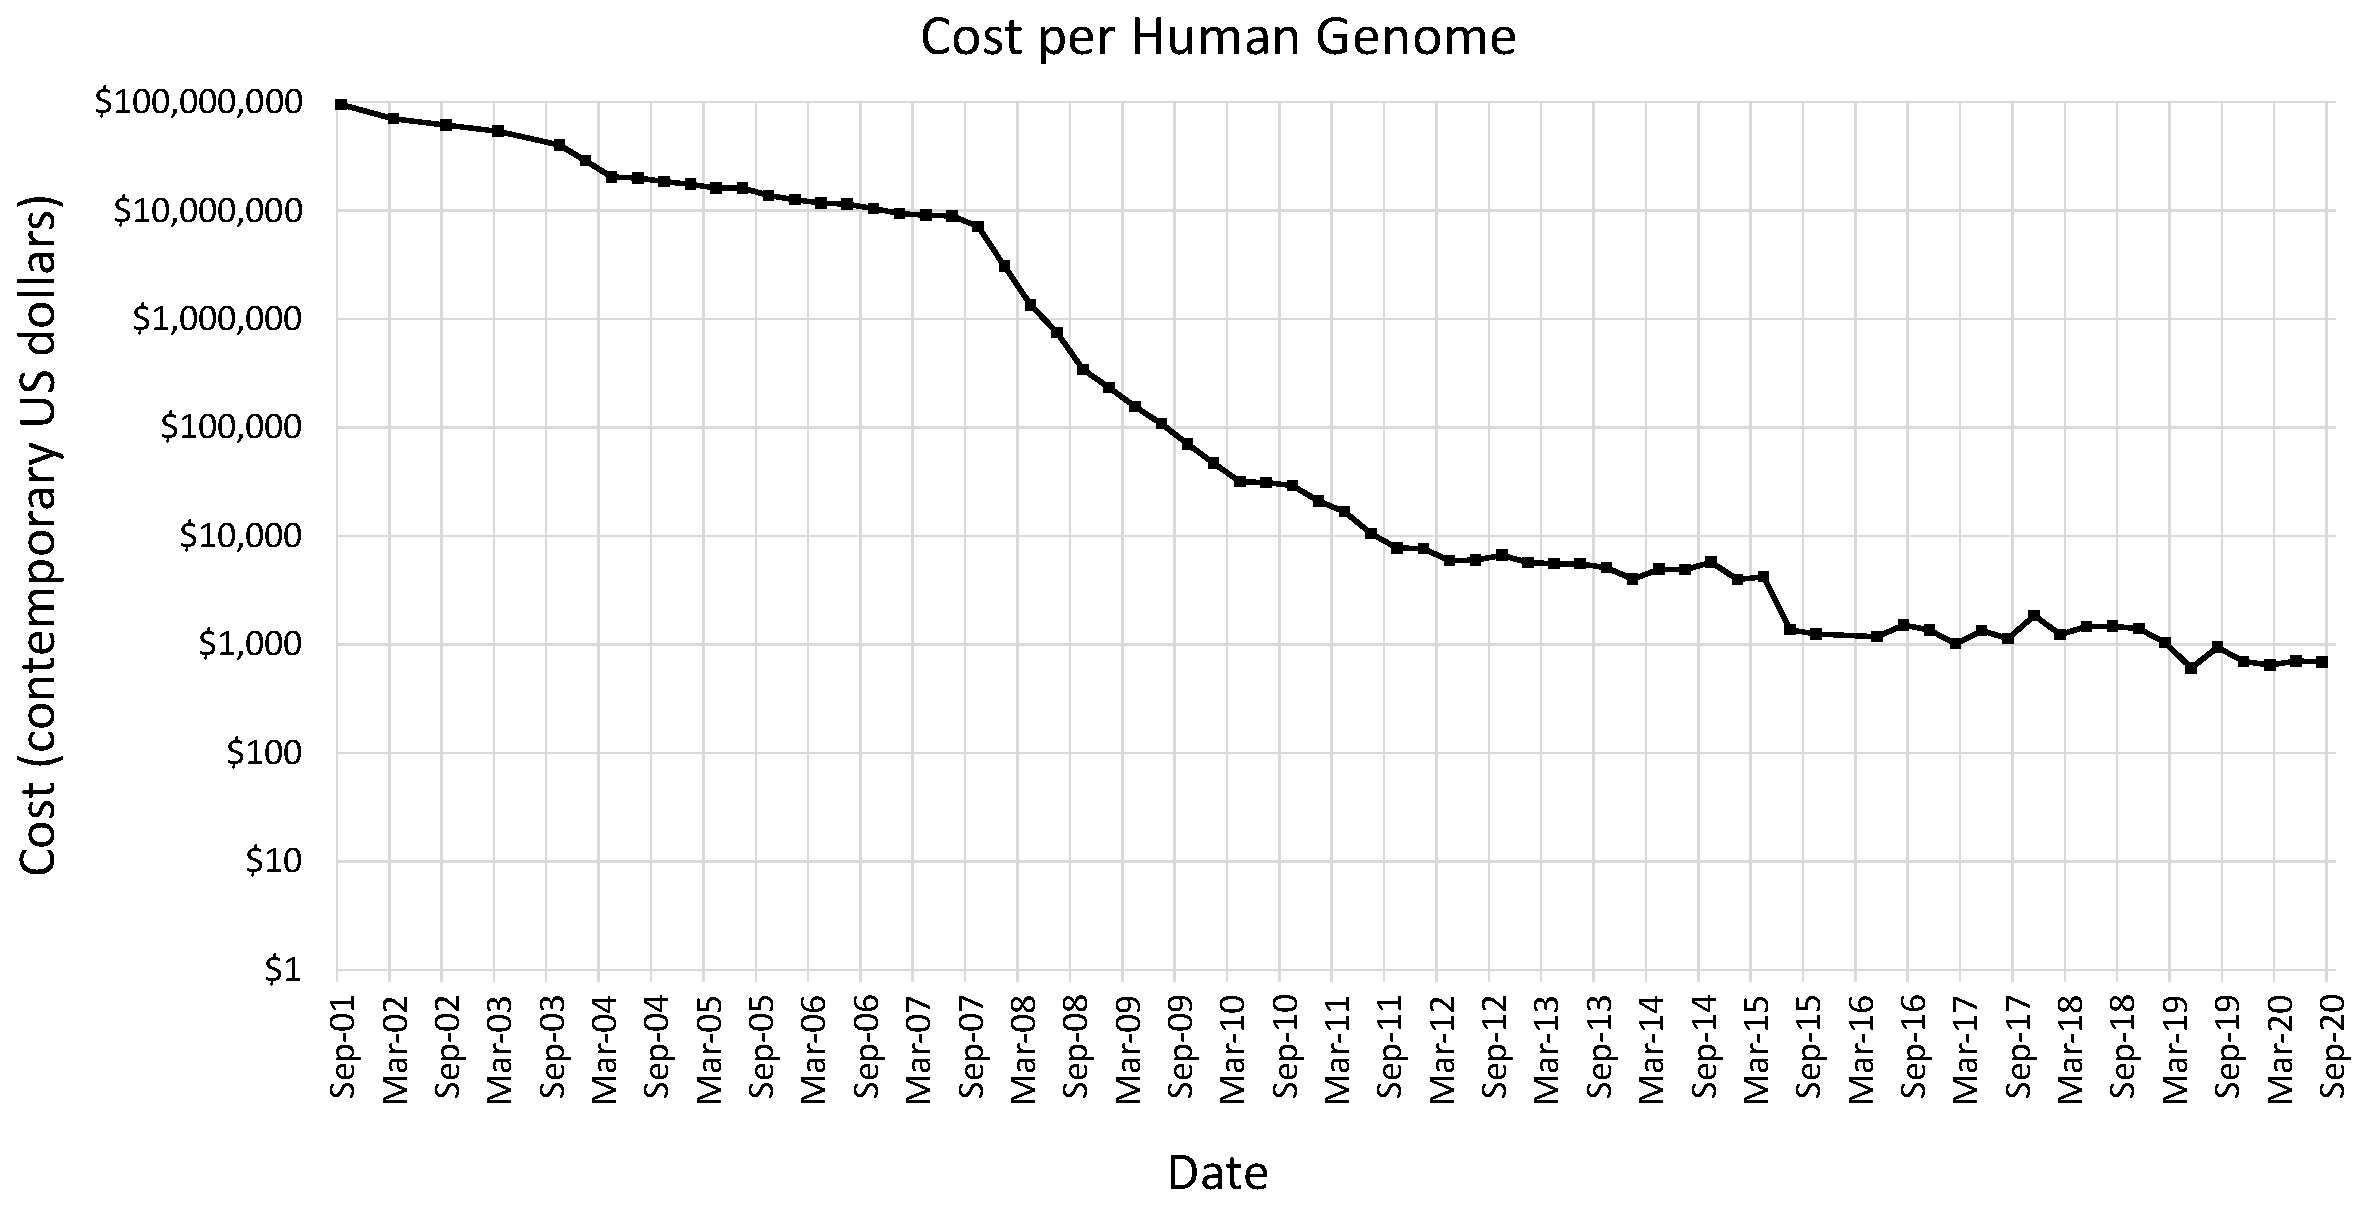
\includegraphics[width=0.95\textwidth,keepaspectratio]{images/intro/sequencing_cost}
    \caption[Cost of human genome sequencing from 2001--2020]{Cost of human genome sequencing from 2001 to 2020. The cost to sequence a single human genome (\textit{i.e.}\ 1\texttimes{} coverage) has declined logarithmically during the 21\textsuperscript{st} century, leading to massive growth in DNA sequencing experiments. Data obtained from the National Human Genome Research Institute (NHGRI) \cite{wetterstrand2020}.}
    \label{fig:intro:sequencing_cost}
\end{figure}
Breakthroughs in DNA sequencing have sharply accelerated in the 21\textsuperscript{st} century, such that the cost to sequence a human genome's worth of DNA has logarithmically decreased (Figure~\ref{fig:intro:sequencing_cost}). This has led to an explosion in sequencing-based science, which has been particularly impactful in cancer research by permitting cost-effective sequencing of patient tumor samples to identify genetic changes, and even facilitated clinical usage of DNA sequencing to guide cancer treatment, prognosis, and prediction \cite{rizzo2012}.

\subsection{Next-generation sequencing}
Central to this explosive growth in DNA sequencing (DNA-seq) has been next-generation sequencing, or NGS\@. Unlike Sanger sequencing, NGS is massively parallel, capable of simultaneous sequencing of millions of DNA fragments automatically \cite{wheeler2008}. This has rendered genome-scale experiments tractable for individual laboratories, and been instrumental in the precipitous decline of sequencing time and costs \cite{vandijk2014}. Additionally, the large quantities of data generated by NGS has made quantitative RNA sequencing (RNA-seq) possible, in which reverse transcriptase is used to generate complementary DNA (cDNA) fragments which are then sequenced \cite{wang2009}. RNA-seq permits high-throughput detection of relative gene expression along with detection of gene rearrangements. NGS can be single-end or paired-end. In single-end sequencing, a certain number of bases of one end of a DNA fragment is read, yielding one sequencing read per fragment. Paired-end sequencing reads bases on both ends of the fragment; though the intervening sequence might not be read the fragment ends remain associated, and two reads are obtained per fragment.

\begin{table}[H]
	\begin{center}
		\begin{tabular}{ccccc}
			& & \textbf{Max read} & \textbf{Max throughput} & \textbf{Error} \\
			\textbf{Platform} & \textbf{Chemistry} & \textbf{length (bp)} & \textbf{per run} & \textbf{rate} \\
			\hline
			\textbf{454} & SBS, pyrosequencing & 1000 & 700~Mb & 1\% \\
			\textbf{Illumina} & SBS, reversible terminators & 300 & 3~Tb & \textless{}1\% \\
			\textbf{SOLiD} & Ligation & 75 & 320~Gb & \textless{}0.1\% \\
			\textbf{Ion Torrent} & Semiconductor & 600 & 15~Gb & 1\%
		\end{tabular}
	\end{center}
	\vspace{-0.3cm}
	\caption[Comparison of major NGS platforms.]{Comparison of the four most popular next-generation sequencing platforms. Statistics for 454 and SOLiD sequencing are from 2016 \cite{goodwin2016}, and data for Illumina and Ion Torrent from 2020 \cite{kanzi2020}. Throughput is measured in base pairs sequenced. SBS: sequencing by synthesis.}
	\label{table:intro:ngs_platform_comparison}
\end{table}
Next-generation sequencing began in 2005 with the pyrosequencing method of sequencing by synthesis developed by 454 Life Sciences \cite{margulies2005}. In 2006, Solexa, Inc.\ (now part of Illumina, Inc.)\ released the Genome Analyzer, which pioneered the reversible terminator method of sequencing by synthesis most popular today \cite{bennett2004,bentley2008}. This was followed by SOLiD sequencing by ligation from Applied Biosciences, Inc.\ (ABI) in 2007 \cite{valouev2008}, and semiconductor sequencing by Ion Torrent in 2010 \cite{rothberg2011}. Each of these four major NGS platforms have advantages and disadvantages (Table~\ref{table:intro:ngs_platform_comparison}) \cite{goodwin2016,kanzi2020}, though here we will focus on the Illumina sequencing platform used in all of the studies we will present.

\begin{figure}[htb]
    \centering
    \begin{subfigure}{0.25\textwidth}
        \includegraphics[width=\linewidth,keepaspectratio]{images/intro/illumina_library_prep}
        \caption{}\label{fig:intro:library_prep}
    \end{subfigure}%
    \hfill%
    \begin{subfigure}{0.73\textwidth}
        \includegraphics[width=\linewidth,keepaspectratio]{images/intro/illumina_library_enrichment}
        \caption{}\label{fig:intro:library_enrichment}
    \end{subfigure}
	\vspace{-0.3cm}
    \caption[Library preparation for NGS.]{Library preparation and target enrichment for next-generation sequencing. (\subref{fig:intro:library_prep}) Genomic DNA is fragmented into short DNA fragments and adapter sequences are ligated to each end. This allows PCR amplification of these sequences with primers complementary to known adapter sequences. These adapters also contain sequences required by the sequencing instrument (for Illumina sequencing, complementary to oligonucleotides on the flow cell) along with a sample-specific sequence which permits multiplexing of multiple biological samples in the same sequencing run. (\subref{fig:intro:library_enrichment}) A sequencing library can be enriched for fragments derived from a desired region of the genome. This is frequently performed using a panel of biotinylated probes complementary to the regions of interest, enabling efficient separation of fragments binding to these probes using streptavidin-coated, metal beads. Source: Illumina, 2017, An Introduction to Next-Generation Sequencing Technology. Used under license from Illumina, Inc. All Rights Reserved.}
    \label{fig:intro:seq_library}
\end{figure}
The first step in Illumina sequencing is library preparation. DNA is extracted from the cells to be sequenced and fragmented (Figure~\ref{fig:intro:library_prep}), often by sonication which mechanically fragments DNA \cite{sambrook2006}. Next, adapter sequences are ligated. For Illumina sequencing, an adapter consists of a constant region termed P5 or P7 (P5 and P7 adapters both necessary in a sequencing run), an index region, and a sequencing primer binding site. To generate the tens to hundreds of nanograms of DNA often necessary for sequencing \cite{aigrain2016}, the DNA is amplified by PCR using primers complementary to the P5/P7 sequences.

Researchers and clinicians are frequently interested in subsets of a genome. For instance, a cancer-focused study or clinical assay may focus on cancer-associated genes such as tumor suppressors and DNA repair genes. In whole exome sequencing, the exons of all known protein-coding genes (collectively termed the exome) are desired \cite{choi2009}. This is achieved by a collection of oligonucleotides (termed a panel) bearing complementary sequence to the desired genome regions and linked to biotin molecules (Figure~\ref{fig:intro:library_enrichment}). The panel is allowed to bind to the library, a process termed hybridization. Streptavidin-coated metal beads are introduced into the solution which strongly bind the hybridized fragments. The beads are extracted by magnetic separation, retaining the fragments of interest (``on-target'') to the exclusion of other DNA fragments (``off-target'').

\begin{figure}[htb]
    \centering
    \hspace{0.5cm}%
    \begin{subfigure}{0.45\textwidth}
        \includegraphics[width=\linewidth,keepaspectratio]{images/intro/illumina_seq_cluster}
        \caption{}\label{fig:intro:illumina_seq_cluster}
    \end{subfigure}%
    \hfill%
    \begin{subfigure}{0.45\textwidth}
        \includegraphics[width=\linewidth,keepaspectratio]{images/intro/illumina_seq_seq}
        \caption{}\label{fig:intro:illumina_seq_seq}
    \end{subfigure}%
    \hspace{0.5cm}
	\vspace{-0.3cm}
    \caption[Overview of Illumina sequencing by synthesis.]{Overview of Illumina sequencing by synthesis. (\subref{fig:intro:illumina_seq_cluster}) To permit sequencing, input DNA fragments must be separated and amplified. This is accomplished by binding of DNA to flow cell oligonucleotides followed by bridge amplification, resulting in multiple clusters of fragments with identical sequence. (\subref{fig:intro:illumina_seq_seq}) The actual sequencing begins with single-stranded DNA clusters adhered to the flow cell, and occurs through multiple cycles by gradually synthesizing a complementary strand. In each cycle, fluorophore-labeled reversible terminators are introduced to extend the new strand by one base, the flow cell is imaged to read the fluorescence signals, and the nucleotide protecting groups are cleaved. Source: Illumina, 2017, An Introduction to Next-Generation Sequencing Technology. Used under license from Illumina, Inc. All Rights Reserved.}
    \label{fig:intro:illumina_seq}
\end{figure}
The DNA is then introduced to the flow cell, a glass substrate coated with two oligonucleoties; one complementary to the P7 adapter sequence, and the other with the P5 sequence. The DNA strands in the library bind to the flow cell (Figure~\ref{fig:intro:illumina_seq_cluster}). The flow cell-bound oligonucleotide is extended by a DNA polymerase to create an entire complementary DNA fragment tethered to the flow cell. Its free end is complementary to the P5 sequence, and binds to a nearby P5 oligonucleotide to create a bridge. The P5 oligonucleotide is extended by DNA polymerase, and the strands again separate. Repeated cycles of this process, termed ``bridge amplification'', creates multiple copies of each flow cell-bound input DNA fragment in the same region (or ``cluster'') of the flow cell \cite{buermans2014}.

The library is now ready for DNA-seq. A solution of modified nucleotides with 3' protecting groups (termed ``reversible terminators'') and fluorophores is added, and the DNA polymerase is able to incorporate one nucleotide  (Figure~\ref{fig:intro:illumina_seq_seq}). The entire flow cell is imaged by a high-resolution camera, yielding a pattern of colored dots in which each dot (corresponding to a cluster) represents a base added to a DNA fragment. In this way, each machine cycle is able to determine a base of millions of fragments at once. After imaging, the protecting groups are removed and new fluorophore-labeled reversible terminators introduced to begin the next cycle. This process repeats for multiple cycles (often 300), generating millions to billions of reads. A flow cell may be divided into ``lanes'' (depending on the specific sequencing instrument), permitting multiple simultaneous NGS experiments per machine run.

\subsection{Emerging sequencing technologies}
DNA-seq techniques and technology remain an active area of research and commercial interest. One notable advance in library preparation is single-cell sequencing \cite{navin2011}. These protocols are capable of uniquely barcoding genomes, genomic regions, or even mRNA molecules from individual cells to permit detailed genomic maps of cell to cell variability. Another innovation in sequencing libraries is the use of UMIs (Unique Molecular Identifiers) \cite{kivioja2012}. The original DNA or RNA sample contains genetic material from multiple cells (except in single-cell experiments). However, the necessary library amplification step also creates duplicate fragments, therefore it is typically impossible to distinguish duplicate fragments derived from different pieces of original DNA from fragments artificially duplicated by PCR or from a single cluster misread as multiple clusters by the imager (optical duplicates). UMIs solve this problem by including short random sequences in different adapter molecules which are later sequenced. This permits computational differentiation between PCR\slash{}optical duplicates and true duplicate original fragments, enhancing the quantitative accuracy of determining the relative abundance of genomic regions which is particularly important for RNA-seq and CNV calling. Technical duplicates can in fact be leveraged through ``consensus calling'', in which multiple reads from the same original fragment are compared to increase confidence in the fragment sequence.

Multiple new sequencing methods have been developed in recent years, collectively termed ``third-generation'' sequencing \cite{vandijk2018}. Leading third-generation methods include PacBio sequencing and Oxford Nanopore. PacBio sequencing (commercialized in 2011) circularizes input DNA fragments and employs a fluorescence-based sequencing by synthesis approach \cite{eid2009}. The circularization step permits each individual fragment to be sequenced multiple times, increasing sequencing accuracy with each revolution of the DNA fragment through the polymerase. Nanopore sequencing (released in 2014) utilizes an entirely different approach; DNA fragments are fed through a membrane containing protein nanopores, and the differing electrical charges of nucleotides are read as each fragment traverses a nanopore \cite{jain2015}. Though these methods have yet to displace Illumina sequencing, they are continuing to mature and have the distinct advantage of generating much longer read lengths (on the order of tens of kilobases) than any NGS platform.

\subsection{Basics of computational analysis}
The end result of next-generation sequencing is a collection of DNA fragments and associated quality scores\footnote{This may require a demultiplexing step which is typically performed by the sequencing instrument.}. These are typically stored in FASTQ format, which for each read contains its assigned name (important for tracking read pairs from paired-end sequencing, and encoding the flow cell position to reduce optical duplicates), the DNA sequence in ASCII-encoded plaintext, and quality scores in Phred format. Phred scores \cite{ewing1998} encode the probability of an incorrect base call as follows:
\begin{equation}
     Q = -10\log_{10}(P_{\text{error}})
\end{equation}

\begin{figure}[htb]
    \centering
    \begin{subfigure}{0.55\textwidth}
        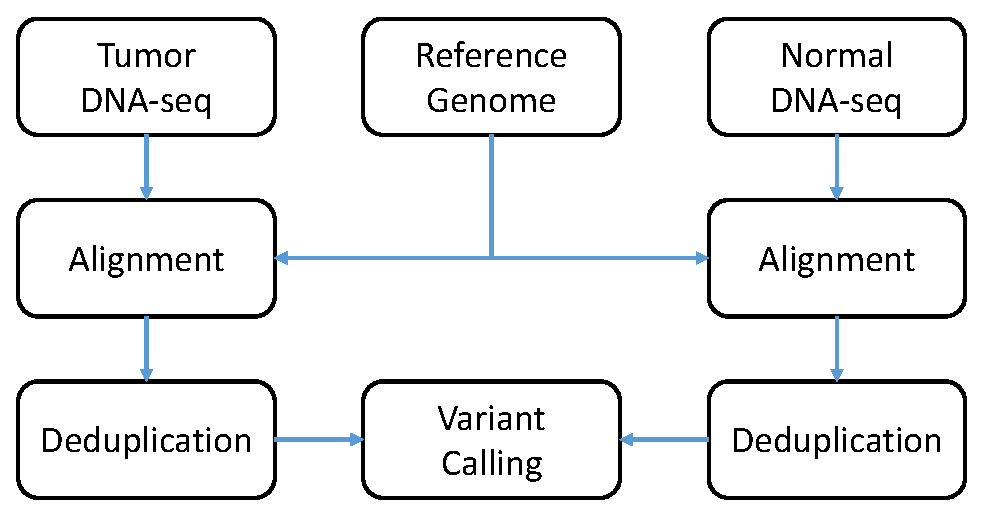
\includegraphics[width=\linewidth,keepaspectratio]{images/intro/info_flowchart_dna}
        \caption{}\label{fig:intro:info_flowchart_dna}
    \end{subfigure}%
    \hfill%
    \begin{subfigure}{0.35\textwidth}
        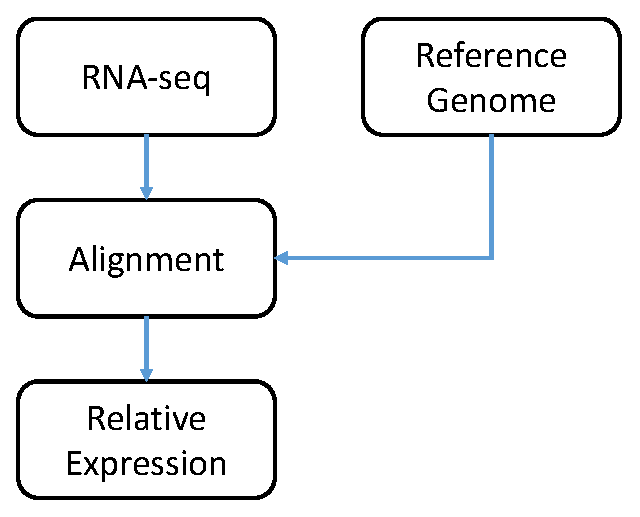
\includegraphics[width=\linewidth,keepaspectratio]{images/intro/info_flowchart_rna}
        \caption{}\label{fig:intro:info_flowchart_rna}
    \end{subfigure}
	\vspace{-0.3cm}
    \caption[Overview of common bioinformatics steps in DNA-seq and RNA-seq.]{Overview of common bioinformatics steps in DNA-seq and RNA-seq processing. (\subref{fig:intro:info_flowchart_dna}) Depicted here is a generic somatic variant calling workflow for cancer genomic analysis, where reads from tumor and normal DNA sequencing are aligned to a reference genome, duplicate reads removed, and somatic variant calling performed. (\subref{fig:intro:info_flowchart_rna}) In this generic RNA-seq experiment, RNA-seq reads are aligned to a reference genome and the relative coverage of exons, transcripts, and genes is computed.}
    \label{fig:intro:info_flowcharts}
\end{figure}
The first analysis step is typically alignment of sequences to the organism's reference genome (Figure~\ref{fig:intro:info_flowcharts}). In the case of humans, the first reference genomes were created by the Human Genome Project and Celera Inc.\ (Section~\ref{ssec:intro:seq_beginnings}). Today, standard reference genomes for human, mouse, rat, zebrafish, and chicken are curated by the Genome Reference Consortium, part of the NIH\@. A variety of software tools have been developed and remain in common use \cite{li2010}. Aligning short reads from NGS to a long reference genome is typically a two-step process. First, the entire genome must be searched for likely hits, for example utilizing hash tables \cite{altschul1990} or graph-based representations of the genome (\textit{e.g.}\ suffix trees \cite{abouelhoda2004}, Burrows-Wheeler transform \cite{burrows1994}). The second step entails semi-global alignment of the read with the sequence near each likely hit, which typically utilizes dynamic programming to achieve $O(mn)$ runtime such as the Needleman-Wunsch algorithm \cite{needleman1970} with zero initial and final gap penalties. Aligners typically output data in the BAM format\footnote{BAM is increasingly being supplanted by CRAM, which encodes the same information but with sequences represented as edits to the reference genome to reduce file sizes.} \cite{samtools}, a block GZIP-compressed representation of read sequences, quality scores, alignments and metadata.
%need to detail DP or alignment more?

After alignment, reads from DNA-seq (but not RNA-seq) must be deduplicated unless UMI-containing adapters were used, to remove optical and PCR duplicates. Typically aligned reads are sorted by position (requiring $O(n\log(n))$ time) and duplicates marked in one pass. Quality control metrics are typically computed, for instance the percent of reads which aligned to the genome or a genomic subset (if a capture panel was used), and the proportion of G/C bases in read sequence. A variety of other bioinformatics methods can be applied depending on experimental conditions and expected biases, for instance end-trimming of reads (as base quality scores typically decline with later sequencing cycles) \cite{martin2011} or normalization of quality scores \cite{mckenna10}.

An enormous variety of analyses have been developed utilizing aligned reads. For DNA, two common downstream analyses are variant calling and CNV calling. Typically variant calling identifies changes in read sequences from the reference genome and performs statistical calls to identify likely SNVs and indels \cite{pirooznia2014}. This can be performed with one sample alone to identify changes from a germline such as population-level SNPs, or with two samples (typically a tumor and matched normal DNA from the same patient) to identify somatic mutations. CNV calling compares the relative quantity of reads at different locations in the genome (the ``coverage'' of these locations) to a copy-neutral reference (usually either a matched normal or pooled panel of normals from multiple individuals) to detect relative gains and losses of genomic regions. A wide variety of tools are available today for variant and CNV calling, implemented using diverse methods of varying levels of sophistication. RNA-seq experiments are typically analyzed to quantify relative gene expression, a process superficially similar to CNV calling of DNA but with unique considerations due to varied splicing of genes \cite{conesa2016}. This can be performed within a single sample, in which expression is typically normalized for gene/transcript length, or between groups of samples in a differential expression experiment to identify genes upregulated or downregulated in one group versus another.

\section{Tumor heterogeneity}
Cancer in humans is an exceptionally complex disease. Considering cancer as a singular `disease' is a misnomer, as human cancer can be classified in a multitude of ways. For instance, cancer is frequently classified by organ site, such as lung cancer, breast cancer, liver cancer, etc. With increasing knowledge of genomics has come the concept of precision medicine, in which clinical decisions are guided by an individual patient's disease \cite{pauli2017}. Taken to its extreme, each case of cancer can be considered a disease of its own, as unique as the genome of the patient. This is termed \textbf{intrapatient heterogeneity} \cite{menzies2014}. But even considering each case of cancer as its own disease fails to fully embody the complexity of cancer, as a single case of cancer in an individual patient may consist of multiple varieties of cancer cells. This is termed \textbf{intertumor heterogeneity}, in which different cancer cells possess different genetics with potential consequences in behavior \cite{marusyk2010}.

\subsection{Concepts}
\begin{figure}[htb]
    \centering
    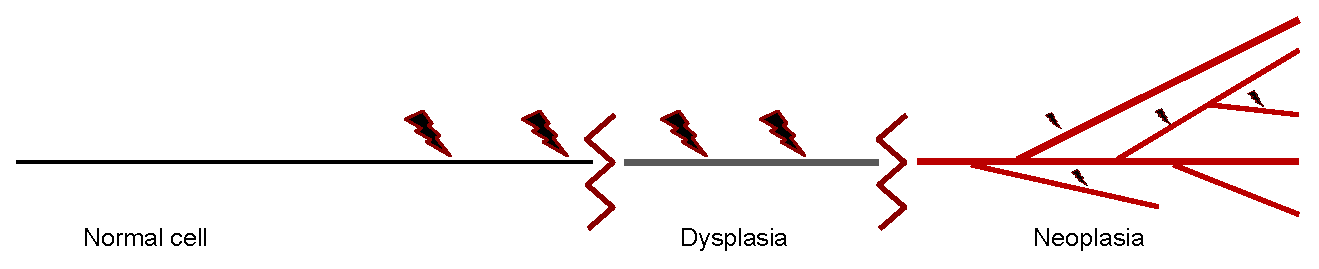
\includegraphics[width=0.95\linewidth,keepaspectratio]{images/intro/heterogeneity_diagram}
    \caption[Tumor heterogeneity arises from cancer mutation.]{Mutations can lead to cancer and intratumor heterogeneity. In a cancer case, the first neoplastic cell arises from mutations acquired in its genetic history. As cancer cells multiply, they have the capacity to diversify as different cancer cell subpopulations acquire different mutations. Lightning bolt symbols represent mutations.}
    \label{fig:intro:heterogeneity_diagram}
\end{figure}
An enormous variety of mutations can lead to cancer in any cell in the human body. Often, normal cells acquire multiple mutations (varying substantially among tumors) and pass through a pre-cancerous dysplastic stage on their way to neoplasia. However cancer cells do not stop mutating; rather each cancer cell is able to acquire mutations and found its own lineages of descendent cancer cells throughout the disease course, which leads to intertumor heterogeneity (Figure~\ref{fig:intro:heterogeneity_diagram}). Intertumor heterogeneity is believed to contribute to several aspects of cancer growth, progression, resistance to treatment, and metastasis \cite{mcgranahan2017}. Freed from the normal constraints on cell proliferation, cancer cells become subject to natural selection in the host organism. Cancer cells which acquire mutations permitting increased growth can grow to outcompete less aggressive cancer cell populations. Some mutations increase the capacity of a cancer cell to metastasize, for example via epithelial-mesenchymal transition \cite{zhang2018}. Metastatic cells encounter a different microenvironment than their tissue of origin, and this new evolutionary fitness landscape promotes microevolution for persistence and survival leading metastatic cancer cells to genetically diverge from the primary \cite{zeeshan2017}.

Tumors encounter opposition throughout their existence. This arises from natural causes, most notably the host immune system, as well as artificial causes \textit{i.e.}\ cancer treatment. To become established and grow, cancer cells must evade or suppress the immune system. However, mutations affecting coding regions of the genome run the risk of creating neoantigens, or immunogenic mutant protein regions which are selected against \cite{vitale2021}. Immune pressure also selects for immunosuppressive mechanisms such as PD-L1 upregulation \cite{kim2016}. Also substantially contributing to tumor heterogeneity are cancer treatments \cite{dagogojack2017}. Many cancer treatments are mutagenic (Section~\ref{ssec:intro:mutation}), producing additional mutations which provide additional chances for tumor microevolution and increased heterogeneity. Treatments also exert selective pressure on tumor cells, as mutations may confer differential sensitivity to treatment by a variety of mechanisms such as (but not limited to) tolerance of chemotherapy, resistance to targeted inhibitors, and escape from ligand dependence. This favors evolution of cells which can grow in spite of treatment, analogous to selection for drug-resistant bacteria with antibiotic therapy.

Single-cell experiments and computational modeling reveal that cancer cells on average acquire multiple mutations per cell division \cite{tsyvina2020,werner2020}. Given that a 1~cm\textsuperscript{3} tumor is estimated to comprise \textapprox{}10\textsuperscript{8} tumor cells \cite{monte2009}, this demonstrates the fantastic potential complexity of tumor heterogeneity. The concept of tumor \textbf{subclones}, first proposed by Dr.\ Peter Nowell in 1976 \cite{nowell1976}, has emerged as a useful paradigm for modeling tumor heterogeneity and evolution \cite{zhu2021}. A subclone represents a population of cancer cells genetically distinct from other subclones; although each cell in a subclone may have genetic differences, all cells in a subclone have genetic similarities characteristic of a common lineage.

\begin{figure}[tbh]
    \centering
    \begin{subfigure}{0.43\textwidth}
        \includegraphics[width=\linewidth,keepaspectratio]{images/intro/heterogeneity_example}
        \vspace{-0.5cm}
        \caption{}\label{fig:intro:heterogeneity_example}
    \end{subfigure}%
    \hspace{1cm}%
    \begin{subfigure}{0.31\textwidth}
        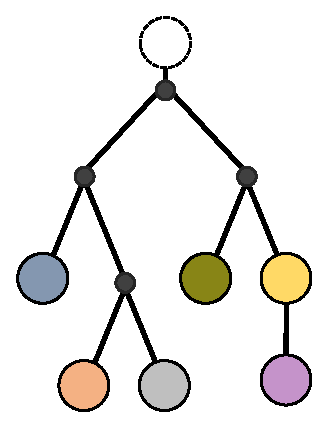
\includegraphics[width=\linewidth,keepaspectratio]{images/intro/tree_example}
        \vspace{-0.07cm}
        \caption{}\label{fig:intro:tree_example}
    \end{subfigure}
    \vspace{-0.3cm}
    \caption[Subclones can approximate intratumor heterogeneity.]{Subclones provide a useful model to approximate tumor heterogeneity. (\subref{fig:intro:heterogeneity_example}) Cancer cells within heterogeneous tumors are grouped into subpopulations termed subclones based on genetic similarity. Subclones are defined for an entire case of cancer, and each circled group of cells represents a separate tumor from a single patient, each comprised of different proportions of subclones. (\subref{fig:intro:tree_example}) Subclonal populations can be organized into a phylogenetic tree reflecting tumor microevolution and acquisition of mutations during the cancer's history. Figure in (\subref{fig:intro:heterogeneity_example}) is based on ``Cancerous cells'' by Les Laboratoires Servier, licensed under CC BY 3.0.}
    \label{fig:intro:subclones_example}
\end{figure}
Through the lens of subclones, intertumor heterogeneity can be approximated by relative proportions of subclonal populations in one or more tumor samples (Figure~\ref{fig:intro:heterogeneity_example}). Differences in subclone abundance among different sites of disease can implicate genes in these subclones as involved in metastasis and metastatic persistence, and shifts over time may reflect responses to treatment and outgrowth of resistant subclones. Furthermore, subclones provide a tractable model of tumor microevolution, as subclonal genotypes can be ordered into an estimated phylogeny (Figure~\ref{fig:intro:tree_example}). Such phylogenies approximate the evolutionary history of each subclone and infer ancestral subclones no longer extant in the available samples, permitting the researcher to estimate the relative timing of mutations during the disease course. Mutations can be divided into ``truncal'' or ``clonal'' mutations which are present in all subclones, and ``subclonal'' mutations found in only some subclones. Cancer treatments targeting truncal mutations may be more efficacious than those targeting subclonal mutations, as in theory all cancer cells would be sensitive (excepting resistance adaptations).

\subsection{Research methods}
\label{ssec:intro:heterogeneity_methods}
Intrapatient heterogeneity has been recognized since the beginnings of cancer treatment, with the observations that different cancers respond differently and possess different prognoses. Advances in cancer research and clinical practice have led to increasingly elaborate classifications of cancer. Currently the World Health Organization (WHO) system is used as a reference standard to classify cancers \cite{who_cancer_classification_1_5,who_cancer_classification_2_5,who_cancer_classification_3_5,who_cancer_classification_4_5}, a scheme which is increasingly incorporating genetic features \cite{carbone2020}. In addition, cancers are classified by stage, the size and extent of cancer in the body, and by grade, the extent of histological differences between tumor tissue and its original tissue type. The American Joint Committee on Cancer (AJCC) curates the TNM (tumor, lymph node, metastasis) system for most human cancer types \cite{amin2017}. However, even these complex classification strategies fail to fully reflect the genetic diversity present among cancers, and the precision medicine paradigm of genomics-guided care is becoming increasingly prevalent \cite{johnson2017}.

Intratumor heterogeneity was first recognized under the microscope, as cancer cells from the same tumor may have widely varying appearances. The genetic basis of intratumor heterogeneity was recognized as early as 1958 through observations of different quantities of genetic material in different cancer cells from the same tumor \cite{huxley1958,mcgranahan2017}. Advances in DNA sequencing and genomics (Section~\ref{sec:intro:genomics}) have provided tools for directly assessing heterogeneous cancer genetics.

The proliferation of NGS along with advancements in bioinformatics have led to the development of a multitude of algorithms to analyze mutation and/or CNV patterns to infer tumor subclones and estimate their evolutionary history \cite{tarabichi2021}. In the following chapters we make use of the software tools Canopy \cite{canopy} and SuperFreq \cite{flensburg2020} and introduce extensions to Canopy (Sections~\ref{ssec:240:subclonal_inference},~\ref{ssec:msiclones:subclonal_msi}). Subclonal inference remains a highly active area of research. In addition, subclonal analysis has yielded genomic findings such as identification of truncal mutations, however such analysis has yet to translate to substantive improvements in clinical practice.

Also key to studies of tumor heterogeneity is sample acquisition. Tumor samples are typically acquired through biopsies. Though clinically routine, biopsies have disadvantages as a research tool. They are invasive and carry clinical risks, such as infection and hemorrhage (often requiring anticoagulant medication to be held, in turn increasing risk of thromboembolism), and they cause inconvenience, discomfort and pain to the patient. A biopsy typically samples only a small portion of a single tumor, which may not be representative of the entire cancer. Such small quantities of tumor tissue also limit the analyses that can be performed. Surgical specimens (such as from resection and debulking surgeries) provide greater quantities of tumor tissue, but not all patients are surgical candidates and surgery may not remove all tumors from a patient.

\begin{figure}[tbhp]
    \centering
    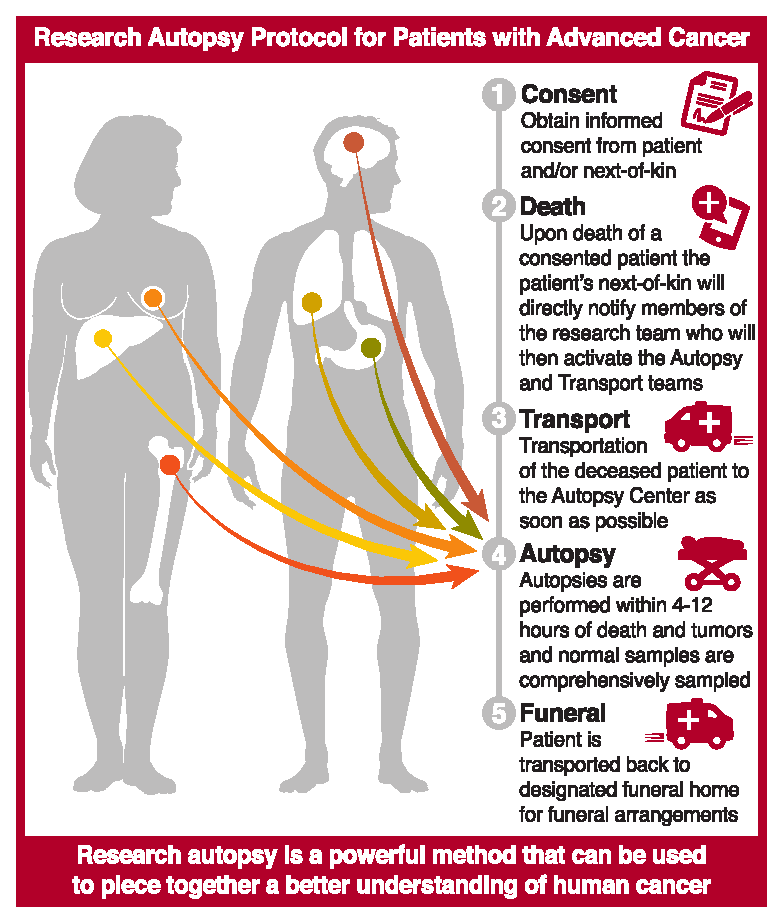
\includegraphics[width=0.7\textwidth,keepaspectratio]{images/intro/autopsy_puzzle_pieces}
    \vspace{-0.3cm}
    \caption[Research autopsy facilitates cancer research.]{Research autopsy facilitates cancer research by providing opportunities for comprehensive tumor sampling and analysis. This allows greater investigation into tumor heterogeneity and evolution, which provides insights into acquired resistance. When performed quickly enough, research autopsy can provide viable cells to create sustainable research resources such as cell lines.}
    \label{fig:intro:autopsy_puzzle_pieces}
\end{figure}
Because of these limitations, research into tumor heterogeneity is increasingly incorporating rapid research autopsy (also called warm autopsy) \cite{duregon2019}. Through collaboration between patients, clinicians, and researchers, patients with advanced cancers and terminal prognosis are provided the opportunity to consent to a rapid research autopsy study (Figure~\ref{fig:intro:autopsy_puzzle_pieces}) \cite{krook2019_review}. Upon notification of death, the decedent undergoes autopsy as soon as possible (ideally within 12 hours post-mortem) to best preserve nucleic acid integrity. A limited autopsy is performed by an on-call team consisting of pathologists and cancer researchers, with reference to previous imaging to extract tumor samples. Special attention is paid during the autopsy such that the patient and their family can receive an open-casket funeral if desired, and that the patient's funeral rites and customs are respected. The decedent is then transferred to the desired funeral home.

Though research autopsy permits comprehensive sampling of large tumor volumes throughout a patient, it can only acquire samples at one time point. Cancer mutates throughout the disease course, and the evolutionary history of tumors at autopsy can at best only be estimated through bioinformatics methods. Therefore, interest is growing in so-called ``liquid biopsies'' through circulating tumor DNA, or ctDNA \cite{merker2018}. Cancer cells release small amounts of their DNA into the bloodstream through a variety of processes, which can be isolated from a blood sample and sequenced \cite{gilson2020}. As blood draws are considerably cheaper, safer, and less invasive than tumor biopsies, ctDNA permits frequent sampling of DNA from tumors throughout the body. However ctDNA typically constitutes a low percent of the cell-free DNA (cfDNA) in the bloodstream and is typically found in very short fragments (even shorter than typically desired for NGS), which poses substantial technical challenges for sequencing and bioinformatics analysis. Additionally, ctDNA permits sampling from multiple tumors in theory, but much remains unknown regarding the relative contribution of different tumors in different locations to ctDNA, which is thought to consist of a complex interaction between genetics, cell turnover, tumor size, vascularity, and other factors \cite{haber2014}. A combination of research autopsy and ctDNA can provide greater insights than either method alone.

%patterns of heterogeneity (linear, branched, neutral, etc)?
%if section needs expanding, possibly subsections Concepts (above), Research Methods (biopsy, histology, autopsy, ctDNA), Current Findings (cite a few clonal papers, mention patterns of heterogeneity)
\section{Cancer as a dynamic process}
As we have seen, cancers acquire mutations throughout the disease course, with potential for substantial impacts on cancer behavior including progression, metastasis, and response to treatment. These in turn affect morbidity and mortality. Though a variety of CLIA (Clinical Laboratory Improvement Amendments)-certified genomics-based tests have been developed such as FoundationOne\textsuperscript\textregistered{} \cite{frampton2013}, Guardant360\textsuperscript\textregistered{} \cite{lanman2015} and OSU-SpARKFuse \cite{reeser2017}, it is impractical to test a patient on a sufficiently frequent basis to gain full awareness of the dynamic mutational landscape of his or her cancer. Even advancements in frequency and ease of testing are frustrated by tumor heterogeneity, which not only substantially increases the complexity of the mutational landscape but renders biopsies and other tumor samples inadequate to study an entire cancer in a patient. To overcome this will require an improved understanding of the temporal and spatial dynamics of cancer mutation, to facilitate empirical and quantitative models that would allow the researcher or clinician to predict and anticipate cancer mutations and their consequent effects on cancer biology. This will require extensive genomic studies, leveraging the power of `Big Data' to permit accurate development and validation of such complicated models.

In this work, we study microsatellite instability, introducing a new algorithm to quantify MSI in tumor samples and the prevalence of MSI across a wide cohort of cancers (Chapter~\ref{ch:msilandscape}). MSI is particularly well-suited to study from a temporal perspective, as MSI-related mutations typically arise at known locations in the genome (microsatellites) and their extent can be efficiently quantified through NGS\@. We provide multiple extensive studies of patients with advanced cancers through NGS and rapid research autopsy, in which we identify tumor subclones and relate these to cancer phenotypic features including treatment resistance (Chapters \ref{ch:240}, \ref{ch:303} and \ref{ch:sclc}). Finally, we develop a framework to quantify MSI within tumor subclones and apply this to a panel of cancers with MSI to quantify microsatellite mutation rates and dynamics in subclonal cancer populations (Chapter~\ref{ch:msiclones}). A fuller understanding of the dynamics of cancer genetics will require substantially greater research efforts, however we hope that the studies presented here will highlight the potential which studies of a cancer as a dynamic process may provide for improved understanding of cancer and clinical management.
